\chapter{Summary and Proposed Work}\label{ch:future}

\section{Summary}

\subsection{Motivation}

The need for this work has been shown by a summary of the current state of the 
art of fuel cycle simulator repository capabilities. The literature review 
concluded that most fuel cycle simulators lack repository analysis beyond basic 
mass tracking. The integrated radionuclide transport and thermal analysis to be 
pursued in this work will provide a currently unavailable tool for disposal 
system analysis. An immediate need for such a tool has been expressed in the 
\gls{UFD} campaign roadmap for this year in which an interface with the \gls{SA} 
campaign was noted as a primary goal. 

\section{Proposed Work}

A repository model, integrated in the \Cyclus fuel cycle simulation platform, 
will be developed in three phases in parallel will supportive \Cyclus 
development. A demonstration phase will implement an `empty' repository 
structure which captures the fundamental software behavior of the subcomponents 
and integrated repository model. A base case phase will build upon the 
demonstration model by implementing the fundamental physics to represent key heat 
and radionuclide transport phenomena for simple unfractured media and canonical  
subcomponent concepts. The final extension phase will build upon the base case 
by implementing extending physics to capture the salient features of various 
competing repository concepts such as fracturation, sorption, and coalescent 
behavior. These phases will be completed within a test-driven software 
development paradigm and will rely on abstractions of the \gls{UFD} \gls{GDSM} 
and \gls{SINDAG} and \gls{LLNL} thermal models.  

\subsection{\Cyclus Framework}

Development of the \Cyclus fuel cycle simulator has generated a tool with which 
the systems analysis aspects of this work will be conducted. Development of the  
fundamental repository module concept appropriate for modular integration with 
\Cyclus has laid the foundation for a software effort which will deliver a 
library of disposal system component models capable of analyzing current 
disposal concepts of interest both domestically and internationally.

\subsection{Demonstration Case Development}

% Demonstration case milestone

A first milestone in the development of this software will be a  proof of 
principle demonstration of the data structure and information passing schemes.  
That is, no physics will be implemented in the demonstration milestone. Rather, 
the component models will be developed in such a way that they are capable of 
passing their information passing schemes and placeholder functions will be 
generated in place of physics.

\subsubsection{Demonstration Case Concept}

  % Concept

    % Facility Interface, complete

    % Control Volumes

    % Dynamic loading

  The demonstration will produce a complete but `empty' repository model. That 
  is, on the repository scale the appropriate facility interface will be 
  implemented, which allows the repository modeled to be loaded into a \Cyclus 
  simulation. A structure of subcomponent control volumes will also be 
  implemented which can be dynamically loaded at runtime.

    % Heat Information Passing

    % Nuclide Information Passing

    % Database writing, structure

  At the subcomponent level, the demonstration will include information passing,
  bookkeeping, and mass and energy balances within and between the subcomponent 
  control volumes.  Information passing between subcomponents concerning heat 
  and radionuclide concentration boundary conditions will be implemented. A 
  complementary output database structure will be defined and bookeeping for 
  writing relevant radionuclide and heat transport information.  

    % basic mass conservation checking

    % basic energy conservation checking


Volumes are defined by their dimensions, surfaces, temperature, contained
matter, and contained contaminants.  Interfaces are defined by a shared 
surface area, a flux type, and a flux direction. Any single volume may only 
interface with one inner and one outer volume. Contained matter must sum 
to the full volume of the volume.

This model treats matter in solid and liquid phases. Gaseous matter is not 
supported. 
Solids are assumed to be porous media and are defined by their porosity 
($n$, $\%$), tortuosity ($\tau$, $[-]$), and dry (bulk) density ($\rho$). 
Early phases of this work will assume just one liquid, water. Later 
extensions will incorporate varying water salinities and chemistries. 
In order to do so, liquids will be defined by their dynamic viscosities ($\mu$, 
[Pascal seconds]),
by characteristic diffusivities ($d_i$, $[m^2/s]$) and solubility ($K$,$[kg/m^3]$) 
coefficients for each nuclide.

\subsubsection{Demonstration Code Development}

  % Code Development
    
  Initial code development on the base case model has begun with creation of the 
  FacilityModel subclass, GenericRepository. This subclass meets the 
  requirements defined by the \Cyclus FacilityModel interface and can be 
  dynamically loaded by the simulator. 

  A first phase in the demonstration milestone will be for the repository model 
  to successfully load its subcomponent models from user input (i.e. the 
  waste form, waste package, buffer, and lithology) with their corresponding 
  defining parameters. A set of parameters that may be sufficient to model the 
  base case is listed in Table \ref{tab:params_tab}.

  %        File: params_tab.tex
%     Created: Thu Aug 18 09:00 PM 2011 C
% Last Change: Thu Aug 18 09:00 PM 2011 C
%
\begin{table}
  \centering
  \footnotesize{
  \begin{tabular}{|l|l|l|l|}
    \multicolumn{4}{c}{\textbf{Initialization Parameters for Subcomponents}}\\
    \hline
    Waste Form & Waste Package & Buffer & Geology \\
    \hline
    \multicolumn{4}{|c|}{}\\
    \multicolumn{4}{|c|}{Inner Radius}\\
    \multicolumn{4}{|c|}{Outer Radius}\\
    \multicolumn{4}{|c|}{Length}\\
    \multicolumn{4}{|c|}{Density}\\
    \multicolumn{4}{|c|}{Specific Heat Capacity}\\
    \multicolumn{4}{|c|}{Initial Temperature}\\
    \multicolumn{4}{|c|}{Heat Transfer Coefficients}\\
    \multicolumn{4}{|c|}{}\\
    \hline
    Porosity           &  Failure Model & Porosity & Porosity \\
    Tortuosity         &                & Toruosity & Tortuosity \\
    Dissolution Model  &                &           &  \\
    \hline
  \end{tabular}
  \caption[Initialization Parameters for Subcomponents]{A preliminary list of 
  user-input initialization parameters for the four primary types of 
  subcomponent models. Some parameters are necessary for all subcomponents.}
  \label{tab:params}
  }
\end{table}




  A second phase will involve implementing an information exchange paradigm 
  between the subcomponents. The purpose of this information passing scheme will  
  be to communicate sufficient temperature fluxes and contaminant concentrations 
  at the boundaries of the control volumes for neighboring subcomponents to  solve 
  their internal transport calculations.  In addition to these Neumann type 
  boundary conditions, additional types of boundary conditions may need to be 
  anticipated.

  When these aspects are implemented, a structure for the output database will 
  be defined and appropriate bookkeeping  will be implemented sufficient to 
  communicate the heat and solute evolution within the repository. 

\subsubsection{Demonstration Testing}

  % Testing

  This work will be developed with a test driven development strategy. That is, 
  before any new functionality is implemented, a suite of tests is written which 
  as closely define its necessary behavior as possible. The software is then 
  written with the goal of passing the test suite. In this way, the software 
  developed in this work is expected to be comprehensively tested in parallel 
  with its development. 


    % Send through 1 radionuclide with no filters in the volumes

    % Have each control volume release 1/3 of what it accepts. see 1/81st.

    Test problems which will help comprehensively define and confirm each unit 
    of the  demonstration functionality will include very basic information 
    passing tests as well as more complex multiple subcomponent integration 
    tests. Every unit of functionality within the model should be tested as an 
    integral part of development.

    A null test of the demonstration case, for example, will release a single 
    contaminant radionuclide through each subcomponent sequentially. This test 
    will pass if  the bookkeeper properly writes to the database its 
    (aphysically unhindered) path through each control volume. Other tests might 
    include a set of database writing tests, subcomponent loading tests, and tests 
    of the facility interface.
    
    When these unit tests pass, validation efforts will take place which show 
    that the complete model behaves in agreement with the more detailed model 
    on which it was based. Else, iterate through sensitivity analyses, model 
    abstraction, and computational development until the model is validated. 


\subsection{Base Case Development}

% Base Case Milestone

The next phase in this work will be the development of the base case. This will 
build upon the demonstration repository module by implementing fundamental 
physics for each of the subcomponents. This will include physically relevant 
mass and thermal balances in each control volume, mixing models that include 
dissolution and solubility limitations as well as fundamental heat  models within 
each subcomponent.  This milestone will result in a repository module capable of
modeling the clay and salt \gls{GDSM} concept modeled by the \gls{UFD} campaign 
and the \gls{ANDRA} and RED-IMPACT  assessments.

\subsubsection{Base Case Concept}

  % Concept

    % uniform unfractured permeable porous medium

      % reducing geochemistry

      The base case concept will model a generic, isotropic, permeable porous 
      geological medium with reducing geochemistry, as well as waste form, 
      waste package, and buffer models in the near field. This model will be 
      appropriate for clay and salt geologies. The fracturation in the geologies  
      of the granite and deep borehole concepts will not be appropriately 
      modeled in the base case unless an equivalent porous medium calculation is 
      conducted external to the code. The incorporation of fracture models will 
      follow in subsequent extensions to the base case.

  
    % WF : glass 

      % alteration

      % temperature limit

    % WF : uox 

      % cladding limit

      % corrosion

      A waste form component module capable of modeling two canonical waste
      form concepts will be developed. It will be modeled with a rate based 
      dissolution model and will be equipped with a heat limit which may 
      constrict the waste form loading. Such a waste form component module will 
      be appropriate for borosilicate glass, the dissolution of which is 
      dominated by a surface alteration rate. It will be appropriate also for a 
      ceramic oxide waste form, the dissolution of which is dominated by a 
      corrosive degradation rate.

\begin{figure}[h!]
\begin{minipage}[b]{0.5\linewidth}
  \begin{center}
    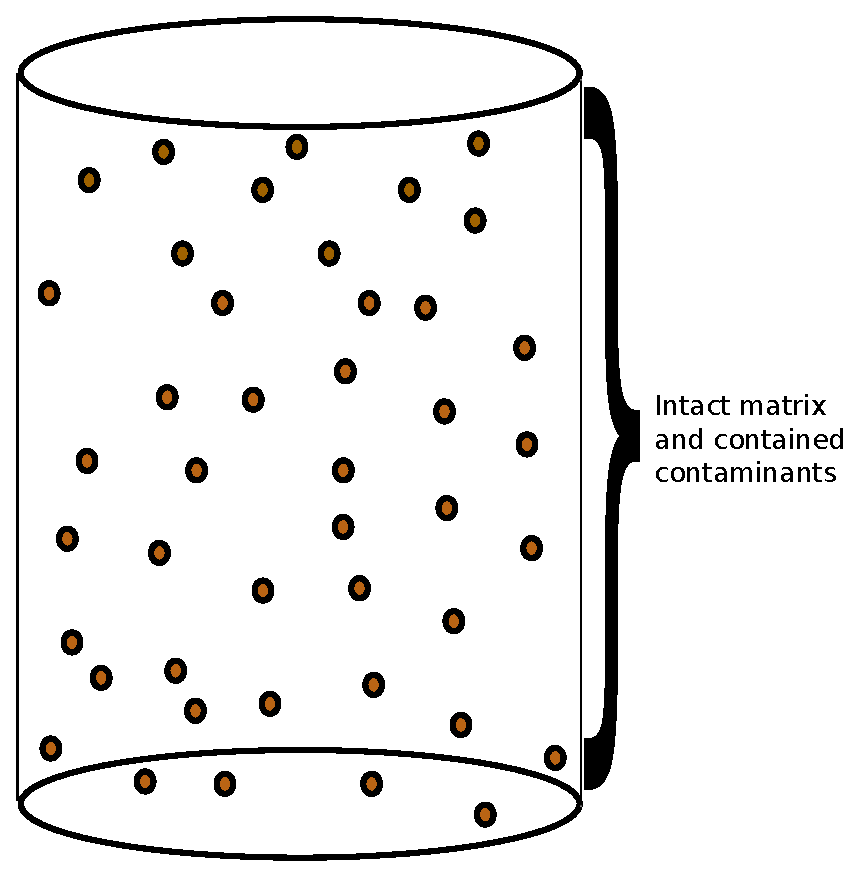
\includegraphics[height=7cm]{./chapters/future/contaminated1.eps}
  \end{center}
  \caption[Intact Waste Form Control Volume]{The control volume contains an intact waste form matrix 
  and contaminants that are unavailable to neighboring subcomponents until 
  dissolution has begun.}
  \label{fig:intact}
\end{minipage}
\hspace{0.5cm}
\begin{minipage}[b]{0.5\linewidth}
  \begin{center}
    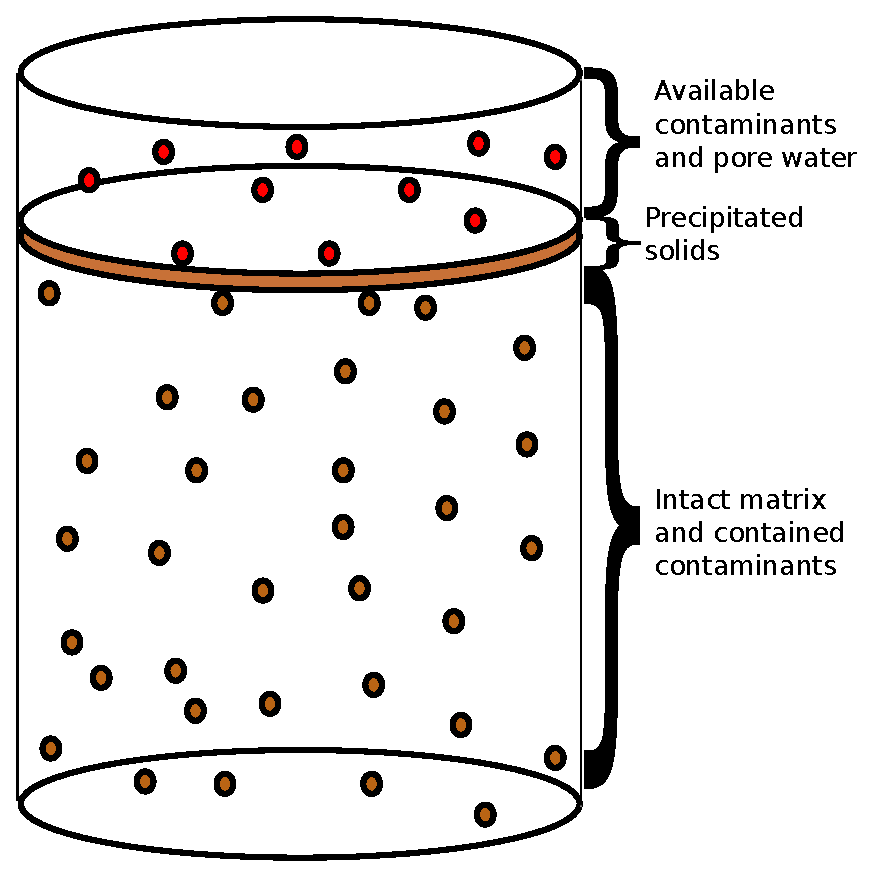
\includegraphics[height=7cm]{./chapters/future/contaminated.eps}
  \end{center}
  \caption[Degrading Waste Form Control Volume]{Once dissolution begins, the control volume contains a partially 
  dissolved waste form matrix, contaminated pore water, and precipitated 
  solids.  }
  \label{fig:dissolved}
\end{minipage}
\end{figure}

    % WP : steel

      % fractional
      
      An explicit time dependent probability distribution waste package failure 
      model will be employed that can accommodate instantaneous, constant, and 
      more complex time dependent failure probability density functions.
      From a user-defined time dependent probability distribution (of which the 
      Weibull distribution might be one), a waste package failure vector will be 
      populated, which assigns a failure time to each waste package object. As 
      the simulation progresses, these waste packages will fail discretely, 
      triggering the initial degradation attack for the waste forms within them. 
      The primary purpose of the waste package model, from a modeling 
      perspective, is to initiate the beginning of waste form dissolution.

    % Buffer : Purely Diffusive Transport 
      
      % permeable porous medium

      The buffer component will be modeled as an isotropic permeable porous 
      medium that is chemically reducing and in which transport is diffusion 
      dominated  and solubility limited.  For the base case, this model will 
      involve only diffusive transport. Extensions to this model will include a 
      model for sorption as well as fracturation and advective transport.  

    % Heat limits at buffer and rock boundary 

      Heat limits in the base case will be calculated at the boundary between 
      the waste package and buffer as well as the boundary between the buffer or  
      backfill and the rock matrix.

\subsubsection{Base Case Abstraction }

  % Regression Analysis

  Abstraction will be conducted for each of the models listed above to identify  
  potential simplifying assumptions.  
  
  Much of this phase of the work will emulate the parametric and regression analysis that
has begun with the base case Clay \gls{GDSM} at \gls{ANL}.  
The Used Fuel Cycle Division has reported sensitivity results for various 
parameters as they affect Peak Annual Dose. Current work has involved a cursory  
exploration of other parameters within the Clay \gls{GDSM} as well. Current 
efforts to repeat those calculations for source term rather than 
dose will provide some insight for the sensitivity of subcomponent models to the 
parameters discussed below. This preliminary analysis has focused on general 
trends and coefficients defining the relationships between these 
parameters and source term over time for each isotope. 

Extending the cooling time between discharge and emplacement results
in an altered waste stream. The resulting source term releases
of this waste stream were expected to differ from base case results. 
Nonetheless it was found that for the clay \gls{GDSM} there was approximately 
no Peak Annual Dose sensitivity to the cooling period length 
\cite{clayton_generic_2011}.

\begin{figure}[h!]
  \begin{center}
    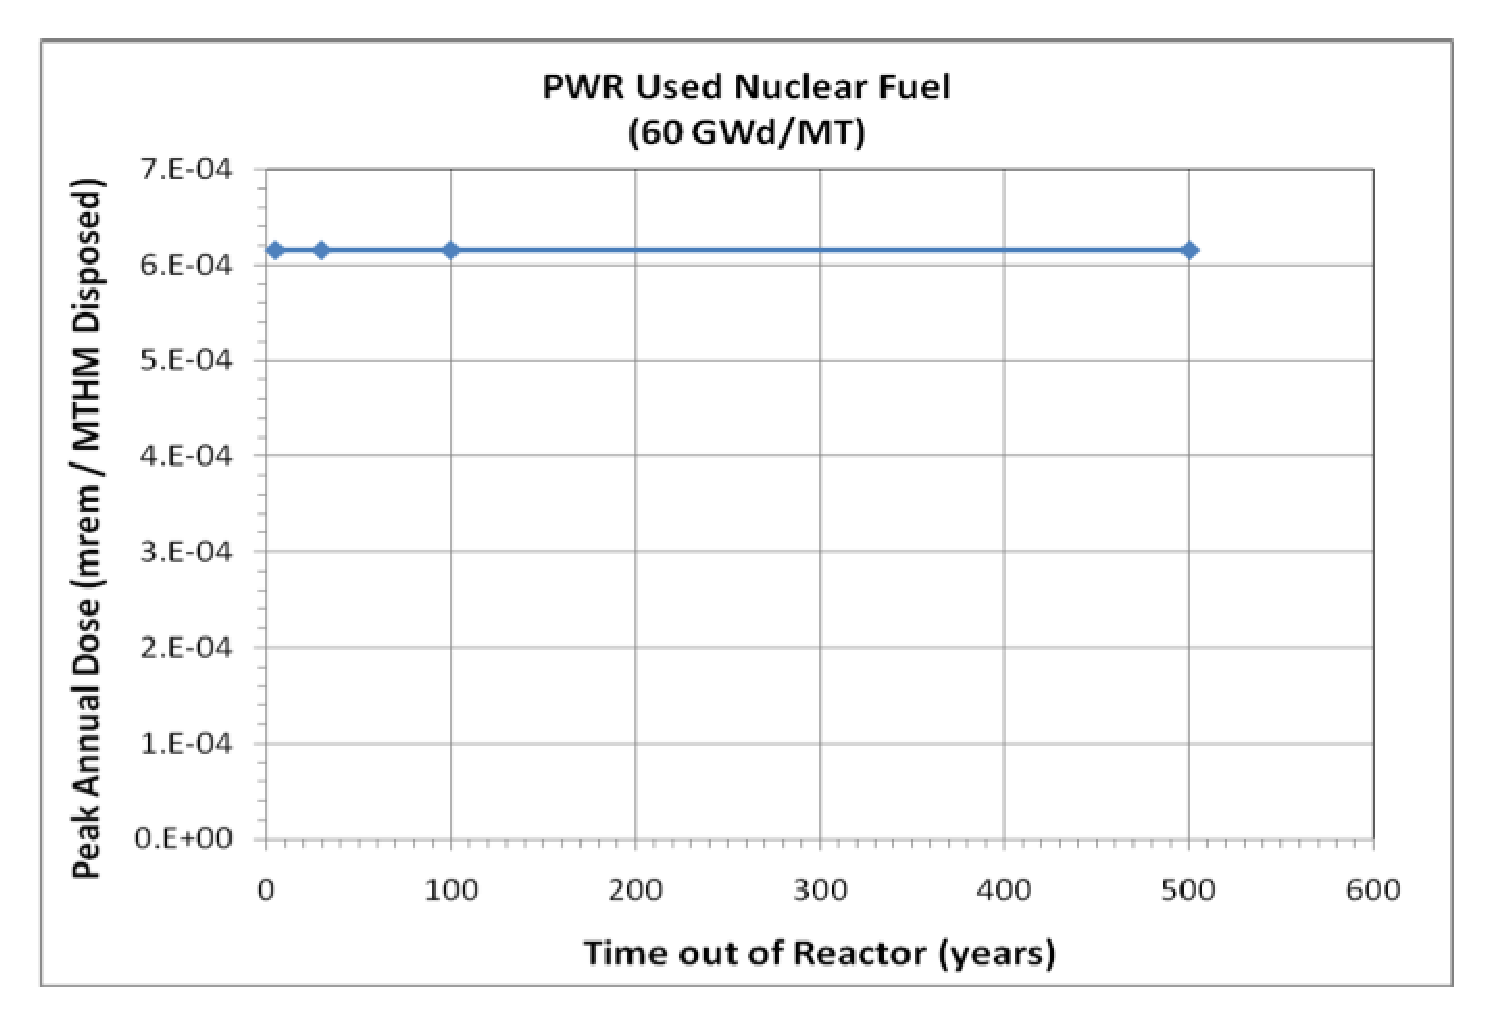
\includegraphics[height=7cm]{./chapters/future/coolingTime.eps}
  \end{center}
  \caption[Cooling Time Peak Dose Sensitivity]{An analysis by the UFD campaign with the clay GDSM shows that
  the peak annual dose is not sensitive at all to the cooling time of a 60GWd 
  burnup PWR fuel \cite{clayton_generic_2011}.}
  \label{fig:coolingTime}
\end{figure}

Since the cooling period will be modeled outside of the repository model within  
the \Cyclus analysis, this sensitivity will not be incorporated into the 
repository modeling effort at the heart of this work, but gives an intuition for 
appropriate sensitivity to altered waste streams.  It is expected that the cooling 
time significantly alters heat based capacity. 


The burnup of a used fuel assembly results in an altered waste stream at the 
time of emplacement. It was found that for the clay \gls{GDSM}, the mean 
annual dose sensitivity to waste form dissolution rate became more important 
linearly with increased burnup \cite{clayton_generic_2011}.


\begin{figure}[h!]
  \begin{center}
    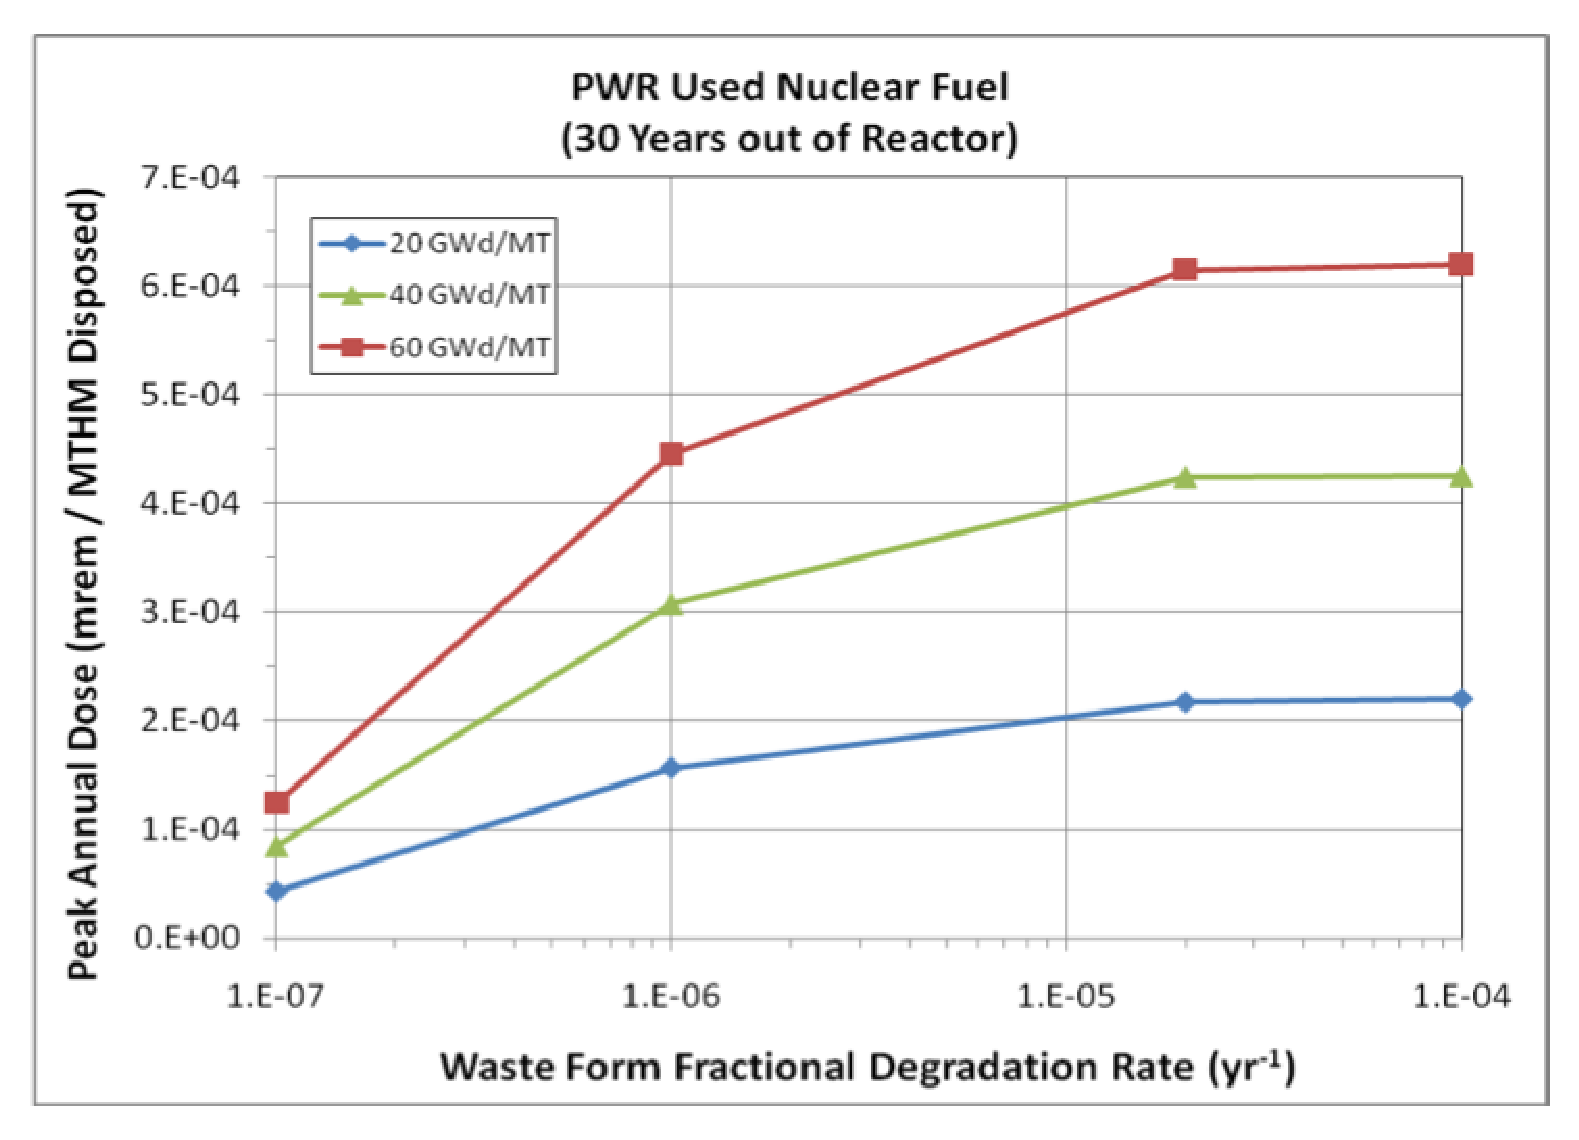
\includegraphics[height=7cm]{./chapters/future/BUandWPdeg.eps}
  \end{center}
  \caption[Burnup and WP Degradation Rate Peak Dose Sensitivity]{An analysis by the UFD campaign with the clay GDSM shows that
  the peak annual dose is more sensitive to waste package degradation rate with 
  increased burnup\cite{clayton_generic_2011}.}
  \label{fig:BUandWPdeg}
\end{figure}
\clearpage

It is expected that the burnup will significantly alter heat based capacity. 
Plutonium and minor actinides are dominant contributors to heat. Focusing on
the sensitivity of the heat based capacity to the waste stream content of 
these radionuclides could significantly simplify the heat analysis. 
 
For each of these, a sensitivity analysis of capacity to the nuclide will be 
developed by analyzing the thermal repository capacity for a waste stream of 
that nuclide alone.  


The mean annual dose has been found to not be very sensitive to the horizontal 
spacing between drifts. However, it is expected that the heat based capacity 
will be highly sensitive to the 
spacing between drifts. A higher drift density produces larger amounts of heat 
generation per repository footprint area. Constrained by heat limits typically 
at the drift tunnel boundaries, the repository capacity is reduced by increased 
areal loading density. 
It is also expected that the heat based capacity will be highly sensitive to the 
spacing between packages linearly within the drifts. A higher line loading 
density produces larger amounts of heat generation per repository footprint 
area.  Again, the repository capacity is reduced by increased areal loading 
density.  It is also expected that the heat based capacity will be highly 
sensitive to the mass loading per waste package. A higher package loading density 
produces larger amounts of heat 
generation per repository footprint area. Constrained by heat limits typically 
at the drift tunnel boundaries, the repository capacity is reduced by increased 
areal loading density. 

The vertical distance to the aquifer above the disposal configuration defines 
the distance separating source term nuclide contaminants from the biosphere. The 
clay model indicates that the mean annual dose is very sensitive to this 
distance \cite{clayton_generic_2011}.

\begin{figure}[h!]
  \begin{center}
    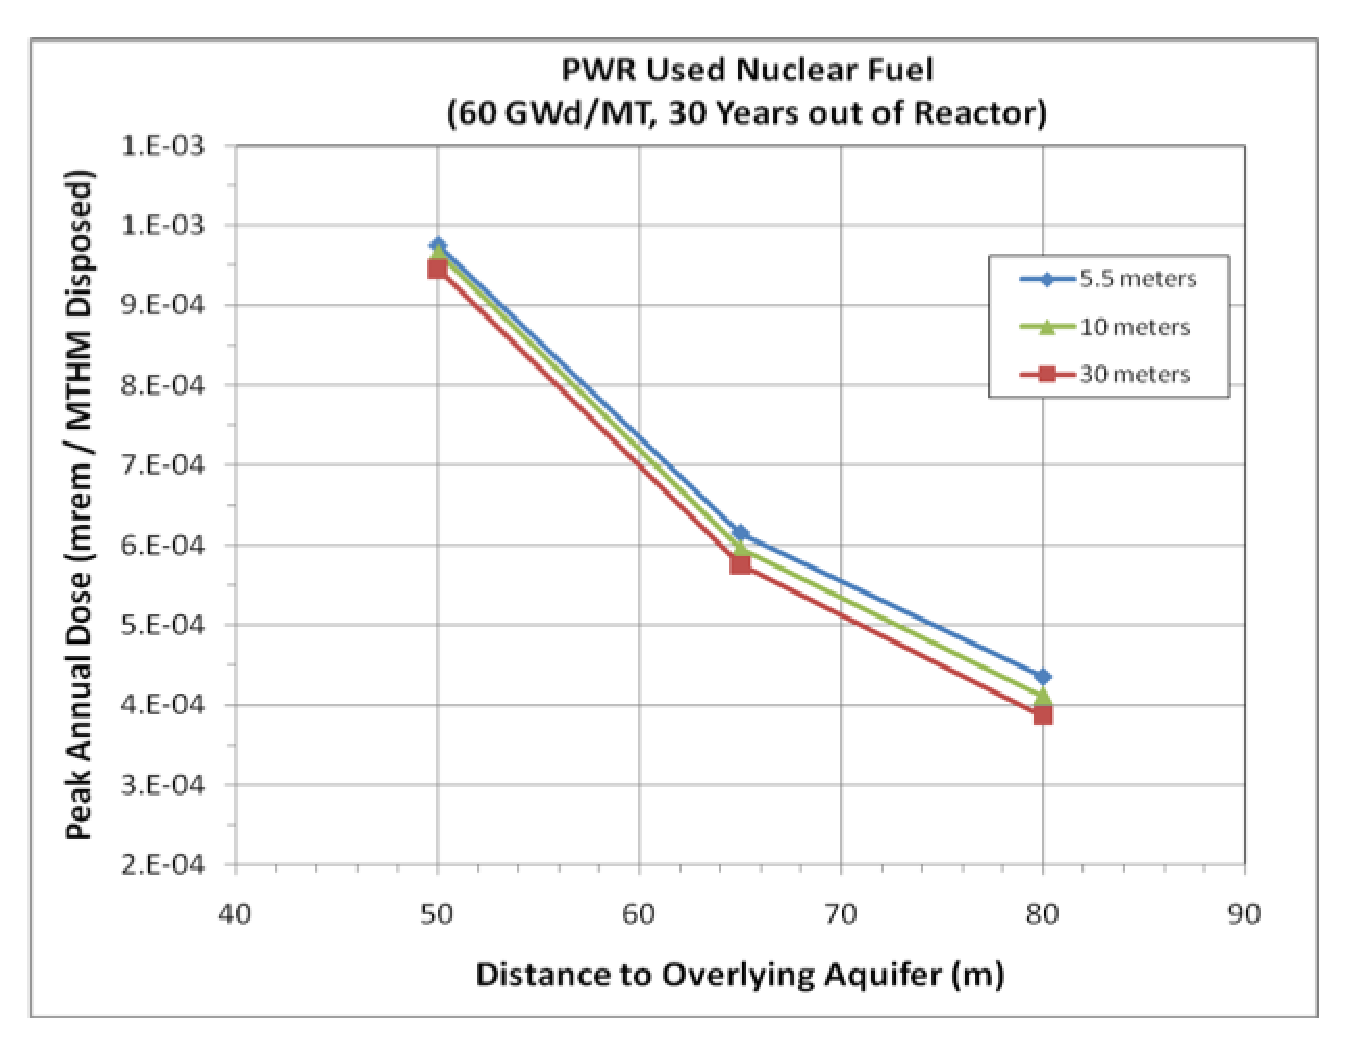
\includegraphics[height=7cm]{./chapters/future/overlyingDist.eps}
  \end{center}
  \caption[Distance to Aquifer Peak Dose Sensitivity]{An analysis by the UFD campaign with the clay GDSM shows that 
  the peak annual dose is very sensitive to the distance to the overlying 
  aquifer\cite{clayton_generic_2001}.}
  \label{fig:overlyingDist}
\end{figure}
\clearpage


Sensitivity to vertical Darcy velocity is similar to the sensitivity to vertical 
distance to aquifer in the sense that it directly determines the nuclide travel 
time to the biosphere. The clay model indicates that the mean annual dose is 
very sensitive to this parameter \cite{clayton_generic_2011}.

\begin{figure}[h!]
  \begin{center}
    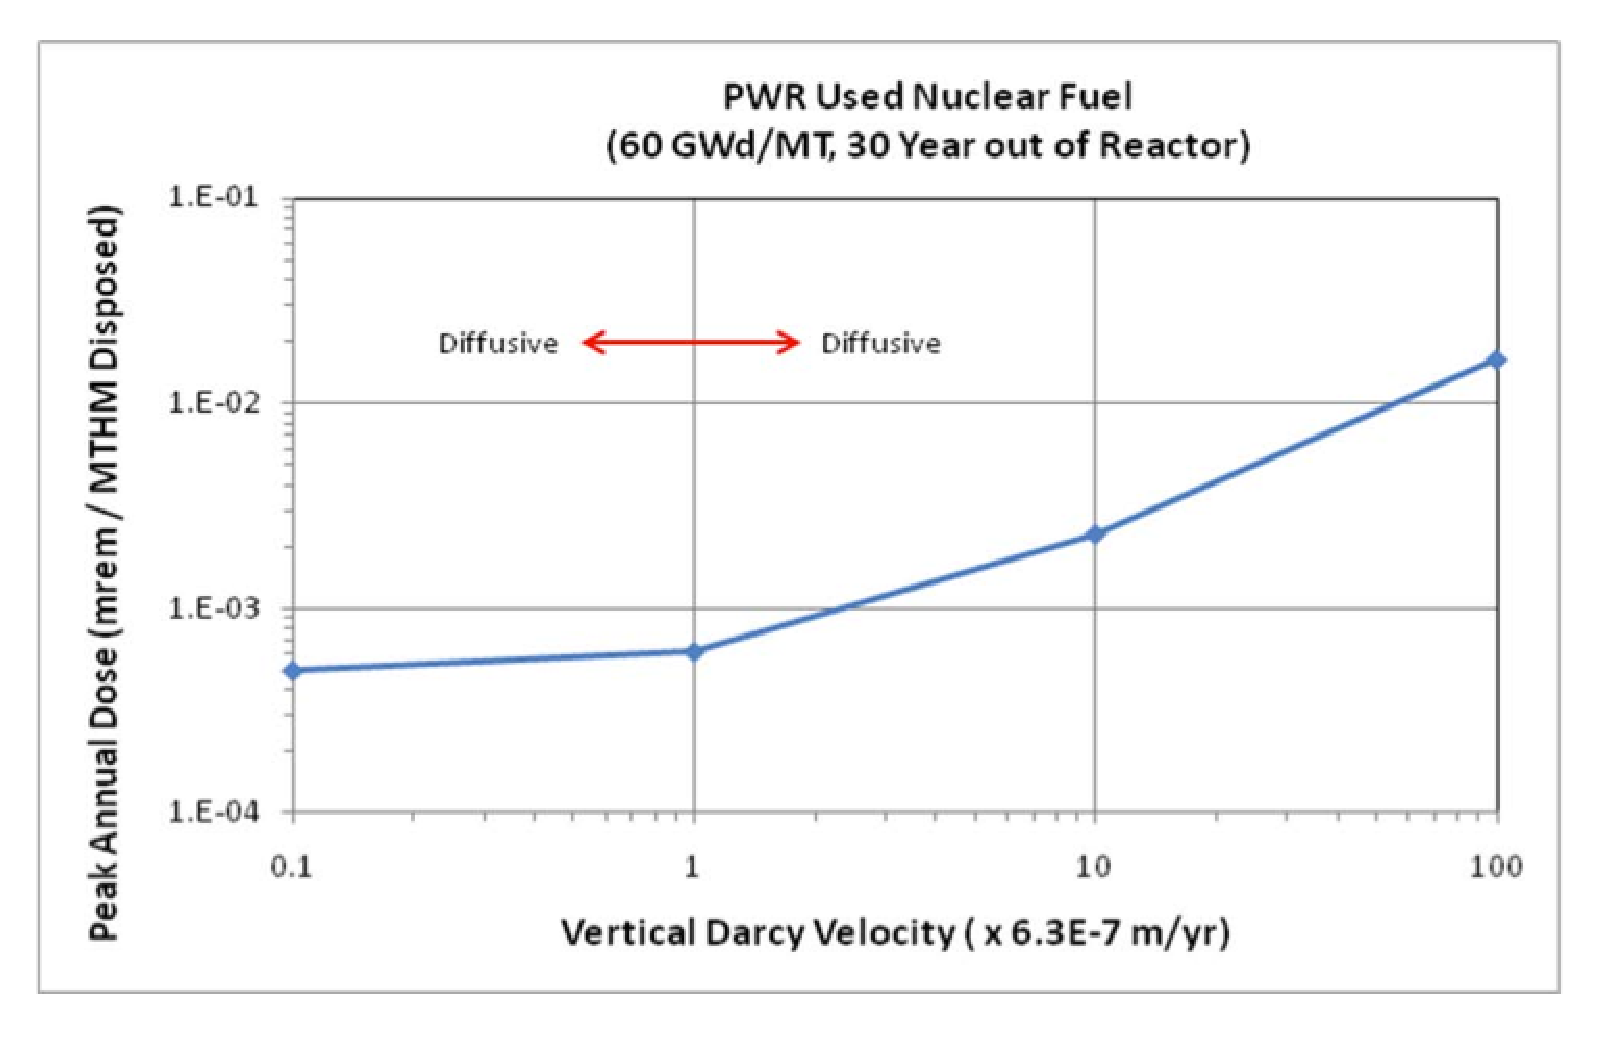
\includegraphics[height=7cm]{./chapters/future/vertDarcyVel.eps}
  \end{center}
  \caption[Vertical Darcy Velocity Peak Dose Sensitivity]{An analysis by the UFD campaign with the clay GDSM shows that 
  the peak annual dose is very sensitive to the vertical Darcy velocity \cite{clayton_generic_2001} .}
  \label{fig:vertDarcyVel}
\end{figure}

\clearpage


Other parameters such as the dimensions of the intersecting fast pathway, the 
permeable porous medium porosity, the waste form and waste package degradation 
rates, will be investigated with the \gls{GDSM} models, the \gls{SINDAG} model, 
and the \gls{LLNL} model. 

\subsubsection{Base Case Code Development}

  % Code Development
  
  Building upon the empty demonstration code stucture, the development of the 
  base case model will primarily consist of populating the subcomponent control 
  volume models with appropriate physics, mass balances, rate equations, and 
  data. This step will implement the calculations in each subcomponent which 
  will provide sufficient information to determine the heat based capacity of 
  the repository for each request of material. 
 
  %        File: cat_table.tex
%     Created: Tue Jul 19 11:00 AM 2011 C
% Last Change: Tue Jul 19 11:00 AM 2011 C
%
\begin{table}
  \centering
  \footnotesize{
  \begin{tabular}{|l|c|c|c|c|c|c|c|}
    \multicolumn{8}{c}{\textbf{Categorization of Phenomena}}\\
    \hline
     Phenomenon&Simplest&&&&&&Hardest\\
    \hline
     WF dissolution&instant&fractional&f(t)&f(H20)&f(T)&f(T,H20)&f(T,H20,etc.)\\
     WP dissolution&instant&fractional&f(t)&f(H20)&f(T)&f(T,H20)&\\
     WF release&instant&fractional&diffusive&advective&diff+adv&congruent&solubility limited\\
     WP release&instant&fractional&diffusive&advective&diff+adv&congruent&solubility limited\\
     Buffer failure&instant&fractional&f(t)&f(H20)&f(T)&f(T,H20)&f(T,H20,etc.)\\
     Buffer release &instant&fractional&diffusive&advective&diff+adv&congruent&solubility limited\\
     FF transport &diffusive&+fractures&+advective&congruent&+sorption&+colloids&solubility limited\\
     WF Heat&indexed&decay&&&&&\\
     WP Heat&conductive&+conv&+rad&+mass&2d&finite diff&finite element\\
     Buffer Heat&conductive&+conv&+rad&+mass&2d&finite diff&finite element\\
     FF Heat&conductive&+conv&+rad&+mass&2d&finite diff&finite element\\
    \hline
  \end{tabular}
  \caption[Categorization of Phenomena]{This table is a preliminary sketch of 
  the various categories of phenomena which will occur in the components of the  
  repository model.}
  \label{tab:cat}
  }
\end{table}



  
\subsubsection{Base Case Testing, Verification, and Validation}

  % Testing
   
  % verification / validation 

  For verification and validation during development, some comparisons to current 
  detailed models such as the \gls{UFD} \gls{GPAM} and GDSMs will be 
  incorporated into the testing framework. Additional verification and 
  validation can be expected to be conducted with respect to known benchmarks 
  such as \gls{ANDRA} and RED-IMPACT results once the model is fully functional.


\subsection{Extensions}

%  Extension Milestone

When the base case is established, a series of extensions to these models will 
be pursued.  This will build upon the base case repository module by 
incorporating sorption, fracturation, coalescence, and disruption 
models within each subcomponent.  This milestone will result in a repository 
module capable of modeling the granite and borehole \gls{GDSM} concepts modeled 
by the \gls{UFD} campaign and the \gls{ANDRA} assessments. Additional extension 
will also incorporate potentially important physical models of salt and clay
coalescent behaviors. 

\subsubsection{Extension Concepts}

  % Concepts

    % Sorption
    
    First, additional phenomena in radionuclide transport will be added to the 
    modeling capability. Sorption, for example, will be added by incorporating 
    sorption effects to the basic diffusive solute transport model, approaching  
    a full solute transport solution such as equation \eqref{ogatabanks}. 
    Additionally, solubility limited transport will be added with a simple 
    restriction on the mixing calculations during mass balancing in the control 
    volumes.

    % Fracturation (granite)
    
    Next, the capability to model fracturation features of granite and borehole 
    geologies will be added  to the modeling capability by adding a dual 
    continuum fracture model.  

    % Coalescent behavior (salt and clay)

    Another anticipated extension will adapt the radionuclide transport model 
    to incorporate the effects of heat and time driven coalescent behavior in 
    clay and salt behavior. This extension will focus on the porosity decrease 
    in those media as time and heat drive collapse around the waste packages.  
    Time dependent coalescence will be addressed first, followed by temperature  
    dependent coalescence.

    % Fast Pathways (borehole and salt)

    A final potential extension may be implemented that will address the issue of 
    modeling a disruption scenario with a fast advective pathway that intersects 
    the repository.  A fast pathway model intended to demonstrate a disrupted 
    scenario is modeled as a single intersecting fracture in the clay matrix. 

\subsubsection{Extension Abstraction}

  % Regression Analysis

  Similar abstraction analysis will be undertaken for the phenomena involved in 
  the extension models. 
  
  For example, the importance of the various 
  ways in which this fast pathway model intersect  the repository is very nuclide
  specific \cite{clayton_generic_2011}. In the clay model the fast pathway intersects the 
  engineered barrier system either directly in the emplaced waste or just outside 
  the secondary engineered barrier system. These details will be analyzed for 
  their importance by regression analysis with the \gls{GDSM} models and 
  iteratively compared to analytical models 

  \subsubsection{Extension Code Development}

  % Code Development

  The code development in the extension phase will follow the same pattern as 
  previous phases, but will focus on extending one feature at a time. 

  \subsubsection{Extension Testing, Verification, and Validation}

  % Testing

  Unit testing, verification and validation will occur in a manner very similar 
  to the previous milestones. Unit tests will assess the performance of each 
  extension functionality as well as their integrated behavior. Validation 
  against \gls{GDSM} results will also be performed for confidence building. 




%
%\paragraph{TAD Canisters} The canisters proposed for transportation, aging and 
%disposal are called TAD canisters.  They are two concentric cylinders of steel 
%and alloy22 inside and out respectively. 
%
%
%\paragraph{Borosilicate Glass} Current borosilicate glass: Includes processing 
%chemicals from original separations, with U/Pu removed, but minor actinides and 
%Cs/Sr remaining Potential borosilicate glass: No minor actinides and/or no 
%Cs/Sr; Mo may be removed to increase glass loading of radionuclides; it has 
%alower volumetric heat rate
%
%
%\paragraph{Glass Ceramic} Glass Ceramic:  This is glass-bonded sodalite from 
%Echem processing of EBR-II, and from potential future Echem processing of oxide 
%fuels o Metal Alloy: This includes subcategories
%
%
%\paragraph{Metal Alloy} Metal alloy from Echem: Includes cladding as well as 
%noble metals that did not dissolve in the Echem dissolution Metal alloy from 
%aqueous reprocessing:  Includes undissolved solids and transition metal fission 
%products
%
%
%\paragraph{Advanced Ceramic} Advanced Ceramic: An advanced waste form that 
%includes iodine volatilized during chopping, which is then gettered during 
%head-end processing of used fuels
%
%
%\paragraph{Separated Streams} Other:  Examples include radionuclides removed 
%from other waste forms (e.g., Cs/Sr, I, C), as well as new waste forms such as a 
%salt waste form
%
%\paragraph{Classes A, B, and C waste} Lower Than High Level Waste (LTHLW): 
%Includes Classes A, ], and C
%
%\paragraph{GTCC LTHLW}  Greater Than Class C (GTCC)
%


\subsection{Fuel Cycle Analysis}

As the model becomes capable of modeling various repository concepts, these will  
be analyzed with relation to canonical closed, open, and modified fuel cycles as  
\Cyclus is capable of them. As discussed before, these fuel cycles will present 
different repository challenges, and analysis with an integrated repository 
model is expected to demonstrate the dynamics of these challenges.   


% UFD developing metrics for the fct program option screening these and perhaps 
% other metrics will be included. 

